\documentclass[aspectratio=169, t]{beamer}
\usepackage[T5]{fontenc}
\usepackage{graphicx}
\usepackage{array}
\usepackage{longtable} % for long table
\usepackage{chngcntr}
\counterwithin{figure}{section}

\renewcommand{\familydefault}{\sfdefault} % Chọn font không chân
% \renewcommand{\familydefault}{\rmdefault} % Chọn font hỗ trợ T5 encoding

\usepackage{caption}
\usepackage{siunitx}

\definecolor{BlueDefault}{rgb}{0.2,0.2,0.7}

% Ẩn navigation (biểu tượng điều hướng)
\setbeamertemplate{navigation symbols}{}

% Thiết lập nền cho các trang nội dung bình thường (được đặt trước khi vào document)
\newcommand{\normalbackground}{%
    \usebackgroundtemplate{
\includegraphics[width=\paperwidth,height=\paperheight]{Source_slides/Normal_page_HUST.pdf}}%
}

\newcommand{\titlebackground}{%
    \usebackgroundtemplate{
\includegraphics[width=\paperwidth,height=\paperheight]{Source_slides/Title_page_HUST.pdf}}%
}

% Đổi màu tiêu đề cho các trang bình thường
\setbeamercolor{frametitle}{fg=white} % Đặt màu chữ title là trắng cho trang bình thường

% Nâng tiêu đề bằng \raisebox
\setbeamertemplate{frametitle}{%
    \vspace{0.3em}
    \hspace{-1em} \insertframetitle
    \vspace{2mm}
}

% Hiển thị số trang ở góc dưới bên phải
\setbeamertemplate{footline}{%
    \hfill % Đẩy số trang sang phải
    \insertframenumber/\inserttotalframenumber
    \hspace{2em} % Tạo khoảng cách từ mép phải
    \vspace{1em}
}

%% Make Table of Contents %%
\AtBeginSection[]{
  \begin{frame}
  \frametitle{Mục lục}
  \tableofcontents[currentsection]
  \end{frame}
}

%% Section numbering %%
\setbeamertemplate{section in toc}[sections numbered]
\setbeamertemplate{subsection in toc}[subsections numbered]


\renewcommand{\figurename}{Hình \thefigure}
\renewcommand{\tablename}{Bảng \thetable}




%%%%% Bibliography %%%%%
\usepackage[backend=biber,style=ieee]{biblatex}
\addbibresource{citation.bib}

\usepackage{url}
\usepackage{hyperref}
\hypersetup{
	colorlinks=true,
	linkcolor=BlueDefault,
	filecolor=BlueDefault,
    citecolor=BlueDefault,
	urlcolor=BlueDefault,
	pdftitle={Overleaf Example},
	pdfpagemode=FullScreen,
}

\begin{document}

\titlebackground

\begin{frame}[noframenumbering]
    \thispagestyle{empty}
    \bfseries
    \begin{flushleft}
        \vfill
        \vspace{10mm}
        \hspace{-2mm} \textcolor{black}{\Large QUẠC QUẠC} \\[1.5em]
        \textcolor{black}{\large Sinh viên thực hiện: Nguyễn Thành Long 20210547} \\[0.5em]
        \textcolor{black}{\large Giáo viên hướng dẫn: PGS. TS Lê Minh Thùy}
        \vfill
    \end{flushleft}
\end{frame}

\normalbackground

\section{Tổng quan}

\begin{frame}{Công nghệ hiện có}
    \vspace{-6mm}
    \begin{columns}
    \column{0.6\textwidth}
        \begin{figure}
            \centering
            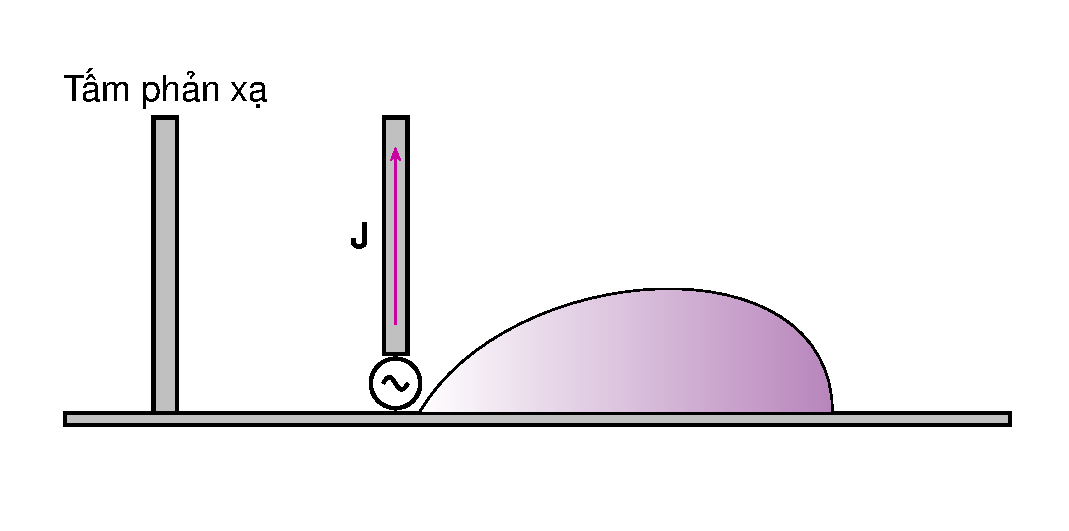
\includegraphics[width=1.0\linewidth]{Figures/Yagi.pdf}
            \caption{Yagi Uda \cite{10818738} \cite{7001061} \cite{7636946}.}
            \label{fig:Yagi_uda}
        \end{figure}
        \column{0.4\textwidth}
        \begin{figure}
            \centering
            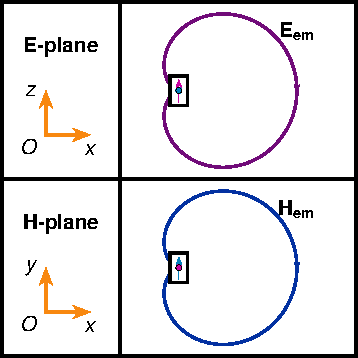
\includegraphics[width=0.75\linewidth]{Figures/MED.pdf}
            \caption{MED \cite{10621581} \cite{7815297} \cite{8753674} \cite{8421283} \cite{9789208}.}
            \label{fig:MED}
        \end{figure}
    \end{columns}
    \begin{itemize}
        \item Tồn tại: bủh bủh lmao.
    \end{itemize}
\end{frame}



\section{Thiết kế}

\input{Slides/Design}

\section{Kết luận và định hướng phát triển}

\begin{frame}{Kết luận và hướng phát triển}
    

\end{frame}

\begin{frame}{Hướng phát triển trong tương lai}
    
\end{frame}



\begin{frame}[allowframebreaks]{Tài liệu tham khảo}
    \printbibliography
\end{frame}

\section{Phụ lục}

\subsection{Bộ tham số tán xạ trong đánh giá mạch cao tần}

\begin{frame}{Bộ tham số tán xạ trong đánh giá mạch cao tần}

\begin{itemize}
    \item Bộ tham số tán xạ \(S\):
\end{itemize}
\begin{equation}
    \left[
    \begin{array}{c}
         V_1^- \\
         V_2^- \\
         \vdots \\
         V_N^-
    \end{array}
    \right]
    =
    \left[
    \begin{array}{cccc}
        S_{11} & S_{12} & \ldots & S_{1N} \\
        S_{21} & S_{22} & \ldots & S_{2N} \\
        \vdots & \vdots & \ddots & \vdots \\
        S_{N1} & S_{N2} & \ldots & S_{NN}
    \end{array}\right]
    =
    \left[
    \begin{array}{c}
         V_1^+ \\
         V_2^+ \\
         \vdots \\
         V_N^+
    \end{array}
    \right]
\end{equation}
hay viết đơn giản:
\begin{equation}
    S_{ij} = \dfrac{V_i^-}{V_j^+} |_{V_k^+ = 0, k \neq j}
\end{equation}
Trong đó,
\begin{itemize}
    \item \(V_{i}^+\) là biên độ sóng điện áp tới cổng \(i\), \(V_{i}^-\) là biên độ sóng phản xạ từ cổng \(i\).
    \item \(S_{ii}\) là hệ số sóng phản xạ tại cổng \(i\), \(S_{ij}\) là hệ số truyền qua từ cổng \(i\) sang cổng \(j\).
\end{itemize}
\end{frame}



\end{document}